%%%%%%%%%%%%%%%%%%%%%%%%%%%%%%%%%%%%%%%%%%%%%%%%%%%%%%%%%%%%%%%%%%%%%%
% writeLaTeX Example: Academic Paper Template
%
% Source: http://www.writelatex.com
% 
% Feel free to distribute this example, but please keep the referral
% to writelatex.com
%%%%%%%%%%%%%%%%%%%%%%%%%%%%%%%%%%%%%%%%%%%%%%%%%%%%%%%%%%%%%%%%%%%%%%
\documentclass[twocolumn,showpacs,%
  nofootinbib,aps,superscriptaddress,%
  eqsecnum,prd,notitlepage,showkeys,10pt]{revtex4-1}

\usepackage{amssymb}
\usepackage{amsmath}
\usepackage{graphicx}
\usepackage{dcolumn}
\usepackage{hyperref}
\usepackage{float}


\begin{document}

\title{Cognitive Services Project}
\author{Stefano Zanatta}
\affiliation{Unipd}

\begin{abstract}
For the \textbf{Cognitive Services - Unipd} Project, I implemented a Deep Convolutional Neural Network (DCNN) with direct connections for image denoising, as described in the Aojia Zhao - Stanford University paper\footnote{\url{https://web.stanford.edu/class/cs331b/2016/projects/zhao.pdf}}, for image denoising.
\end{abstract}

\maketitle

\section{Introduction}
\label{sec:introduction}
This project involves the implementation of the DCNN for image denoising\footnote{\url{https://web.stanford.edu/class/cs331b/2016/projects/zhao.pdf}} described in the abstract, toghether with the analisys of the results and the comparison with the state of the art image denoisers.\\
While classic image denoisers have fully connected layers, the Aojia Zhao one does not have any, reducing the required weights of the model. To further reduce the required weights, this model uses direct connections between each Conv layer and its relative Deconv layer.\\
The implementation of the project can be found in the footnote \footnote{\url{https://colab.research.google.com/drive/14dAdoKLWbCKEJStnLlHphoO-L2mhsVTG}}.

\section{Technologies}
\label{sec:technologies}

\subsection{Google Colab}
\label{subsec:colab}

The project was developed entirely on Google's Jupyter notebook environment, Google Colab. This platform offers many advantages:\\
\begin{itemize}
    \item Code hosted on the Cloud, allowing portability between home, stage and university's computers;
    \item Code executed by Google's servers, allowing more computational power than a traditional Computer;
    \item Free GPU, for ~10 time faster execution than a CPU (experimented during Cognitive Services class);
    \item Python environment, with built in machine learning APIs;
\end{itemize}
During the development of the project, I found some downsides:\\
\begin{itemize}\label{subsec:colab:downsides}
    \item Dataset size and model complexity (e.g. images size, batch size, number of epochs) are limited by the RAM limit of 12GB (within one execution). \textit{This problem is discussed in the dataset section\ref{subsec:dataset}.}
\end{itemize}

\subsection{Keras}
Keras is the main API used for the project, using Tensorflow as backend. Keras offers a simpler interface than Tensorflow, making the process of building the model, training and showing the results easier.  

\subsection{Dataset}
\label{subsec:dataset}
In the table\ref{tab:dataset} are listed the dataset used for each experiment. As mentioned in the Google Colab section\ref{subsec:colab:downsides}, the limited RAM defined the size of the following parameters (higher definition = fewer examples or less epochs).\\
A first experiment with a high definition image saturated the RAM with few epocs, with a validation accuracy of 0.20. For this reason that experiment was not included in the analisis.
\begin{table}[H] \label{tab:dataset}
    \centering
    \begin{tabular}{l|c|c|c|c|c|c}
    \#         & Train           & val/tot\* & Test       & size       & batch size & epochs \\\hline
    1          &  4000           & 0.2      &  375       &  128x128    & 10   &  35 \\\hline
    2          &  11000          & 0.1      &  375       &  64x64      & 10     &  100
    \end{tabular}
    \caption{\label{tab:widgets}Dataset for the different experiments}
    \end{table}
\textit{* val/tot indicates the validation images / total training images ratio}

% Commands to include a figure:
%\begin{figure}
%\includegraphics[width=\textwidth]{your-figure's-file-name}
%\caption{\label{fig:your-figure}Caption goes here.}
%\end{figure}

\subsection{Model}
The model consists of 5 Convolutional (Conv) layers and 5 Deconvolutional (Deconv) layers. Each layer is connected to the following one (e.g. Conv2 with Conv3).\\
Direct connections are implemented by adding the output of a Conv layer with the output of the "opposite" Deconv layer (e.g. Conv2 with Deconv3), and using that result as the input of the next Deconv layer (e.g. Conv2 + Deconv3 is the input of Deconv4 ). This connections are better described by this image todo. 
\begin{itemize}
    \item \textbf{Input:} ($64\times64\times3$) single input of the DCNN, image of 64x64 pixels x3 dimensions (RGB);
    \item \textbf{Conv1:} ($64\times64\times64$) Conv filters of the same dimensions of the input; connected with Conv2 and Deconv4;
    \item \textbf{Conv2:} ($32\times32\times128$) same filters, sizes are halved; connected with Conv3 and Deconv3;
    \item \textbf{Conv3:} ($16\times16\times128$) connected with Conv4 and Deconv2;
    \item \textbf{Conv4:} ($8\times8\times256$) connected with Conv5 and Deconv1;
    \item \textbf{Conv5:} ($4\times4\times512$) doubled filters, image sizes are halved. At this point, the model has many small filters and the image is "deeply encoded". The Deconv layers have to decode the image;
    \item \textbf{Deconv1:} ($8\times8\times256$) from now on, the filter sized are the same of the "opposite" Conv layer, to match the SUM between the two layers;
    \item \textbf{Deconv2:} ($16\times16\times128$) connected with Deconv3;
    \item \textbf{Deconv3:} ($32\times32\times64$) connected with Deconv4;
    \item \textbf{Deconv4:} ($64\times64\times32$) connected with Deconv5;
    \item \textbf{Deconv5:} ($64\times64\times3$) last layer. The image is decoded to the original size and color space.
\end{itemize}


\subsection{Training}
Training was done on two datasets\ref{subsec:dataset}, $128\times128$ and $64\times128$ images. The 128 images required much more resources then the 64 ones, this required reducing the epochs and the number of training dataset.\\
MSE was used as the minimization function in both cases, and the categorical\_accuracy for evaluating the model (the default accuracy for keras).
\begin{table}[H] \label{tab:training}
    \centering
    \begin{tabular}{l|c|c|c|c|c|c}
    Experiment       &  Validation acc & Test acc \\\hline
    1          &  0.7067           & todo            \\\hline
    2          &  todo 75        & todo    
    \end{tabular}
    \caption{\label{tab:widgets}Training results}
    \end{table}

\subsection{Experiment 1}
$128\times128$ images were used for the first experiment, using doubled the size required from the Zhao paper. This quickly saturated the RAM, so reduced the dataset elements and the epochs by more than 50\%.\\
Using 35 epochs, the model stabilized on 0.70 accuracy after few epochs. Changing epocs did not change this result. This probably means that increasing the complexity of the model is required to fit bigger images. This is not possible with Google Colab resources, for the RAM and GPU limits.\\
\begin{figure}[H]
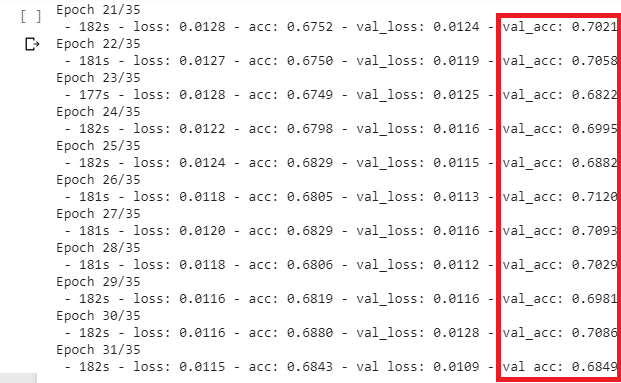
\includegraphics[width=\textwidth]{images/128x128_35epoch_10batch_fit.png}
\caption{\label{fig:your-figure}Training results for experiment 1}
\end{figure}

\subsection{Experiment 2}\label{subs:ex2}
$64\times64$ images were used for the second experiment, as suggested in the Zhao paper. The training was done on 11000 training images, 1100 of them are used for validation.\\
Experiment2 showed better results than Experiment 1, because the accuracy did not saturate at 0.70, but it keept increasing with the epochs.

\subsection{Results}
Even if the model reached just an accuracy of about 0.75, the model could probably reach better results with doubled epochs (around 9 hours of training).\\
The batch size of 10 avoided overfitting. In fact, in the first experiments, increasing the batch size implied a faster growth of the train accuracy, but reduced the validation accuracy.
As i mentioned in the Experiment2 section\ref{subs:ex2}, the model is made for small images, so just for research purposes. Increasing the model complexity would allow to use bigger images, but at the cost of GPU power.

\subsection{Comparison with state of the art models}
To understand how a state of the art models works, i took \textbf{Xiao-Jiao Mao, Chunhua Shen, Yu-Bin Yang's project}\footnote{\url{https://arxiv.org/pdf/1606.08921v3.pdf}} as banchmark. They worked with bigger images, days of training, bigger models (30 layers instead of 10) and different evaluating methods, but still using a DCNN with direct connections.\\
This paper suggests to use small filter size, in fact the filters in the Zhao DCNN were reduced from 64x64 to 4x4. 

\begin{acknowledgments}

We thank\dots

\end{acknowledgments}

\end{document}